\chapter{Fractional Reserve Insanity}
\label{les:13}

\begin{chapquote}{Lewis Carroll, \textit{Alice in Wonderland}}
Alas! it was too late: she went on growing and growing, and very soon had to
kneel down: in another minute there was not room even for this, and she tried
the effect of lying down, with one elbow against the door, and the other arm
curled round her head. Still she went on growing, and as a last resource she put
one arm out of the window, and one foot up the chimney, and said to herself
\enquote{now I can do no more—what will become of me?}
\end{chapquote}

Value and money aren't trivial topics, especially in today's times. The
process of money creation in our banking system is equally non-trivial,
and I can't shake the feeling that this is deliberately so. What I have
previously only encountered in academia and legal texts seems to be
common practice in the financial world as well: nothing is explained in
simple terms, not because it is truly complex, but because the truth is
hidden behind layers and layers of jargon and \textit{apparent} complexity.
\enquote{Expansionary monetary policy, quantitative easing, fiscal stimulus to
the economy.} The audience nods along in agreement, hypnotized by the
fancy words.

Fractional reserve banking and quantitative easing are two of those
fancy words, obfuscating what is really happening by masking it as
complex and difficult to understand. If you would explain them to a
five-year-old, the insanity of both will become apparent quickly.

Godfrey Bloom, addressing the European Parliament during a joint
debate, said it way better than I ever could:

\begin{samepage}\begin{quotation}
\enquote{[...] you do not really understand the concept of banking. All the
banks are broke. Bank Santander, Deutsche Bank, Royal Bank of
Scotland --- they're all broke! And why are they broke? It isn't an
act of God. It isn't some sort of tsunami. They're broke because we
have a system called 'fractional reserve banking' which means that
banks can lend money that they don't actually have! It's a criminal
scandal and it's been going on for too long. [...]
We have counterfeiting --- sometimes called quantitative
easing --- but counterfeiting by any other name. The artificial
printing of money which, if any ordinary person did, they'd go to
prison for a very long time [...] and until we start sending
bankers --- and I include central bankers and politicians --- to
prison for this outrage it will continue.}
\flushright -- Godfrey Bloom\footnote{Joint debate on the
banking union~\cite{godfrey-bloom}}
\end{quotation}\end{samepage}

Let me repeat the most important part: banks can lend money that they
don't actually have.

Thanks to fractional reserve banking, a bank only has to keep a small
\textit{fraction} of every dollar it gets. It's somewhere between 0 and 10%,
usually at the lower end, which makes things even worse.

Let's use a concrete example to better understand this crazy idea: A
fraction of 10\% will do the trick and we should be able to do all the
calculations in our head. Win-win. So, if you take \$100 to a
bank --- because you don't want to store it under your mattress --- they
only have to keep the agreed upon \textit{fraction} of it. In our example that
would be \$10, because 10\% of \$100 is \$10. Easy, right?

So what do banks do with the rest of the money? What happens to your \$90? They
do what banks do, they lend it to other people. The result is a money multiplier
effect, which increases the money supply in the economy enormously
(Figure~\ref{fig:money-multiplier}). Your initial deposit of \$100 will soon
turn into \$190. By lending a 90\% fraction of the newly created \$90, there
will soon be \$271 in the economy \cite{wiki:money-multiplier}. And \$343.90 after that. The money supply is
recursively increasing, since banks are literally lending money they don't have.
Without a single Abracadabra, banks magically transform \$100 into one thousand
dollars or more. Turns out 10x is easy. It only takes a couple of lending
rounds.

\begin{figure}
  \centering
  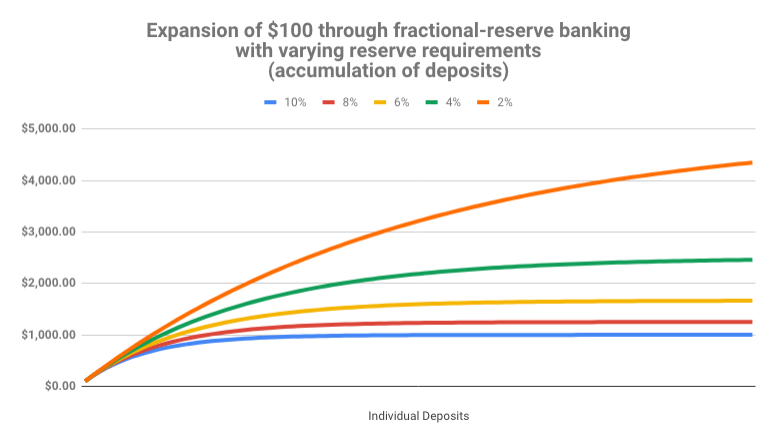
\includegraphics{assets/images/money-multiplier.png}
  \caption{The money multiplier effect}
  \label{fig:money-multiplier}
\end{figure}

Don't get me wrong: There is nothing wrong with lending. There is
nothing wrong with interest. There isn't even anything wrong with good
old regular banks to store your wealth somewhere more secure than in
your sock drawer.

Central banks, however, are a different beast. Abominations of financial
regulation, half public half private, playing god with something which
affects everyone who is part of our global civilization, without a
conscience, only interested in the immediate future, and seemingly
without any accountability or auditability (see Figure~\ref{fig:bsg}).

\begin{figure}
  \centering
  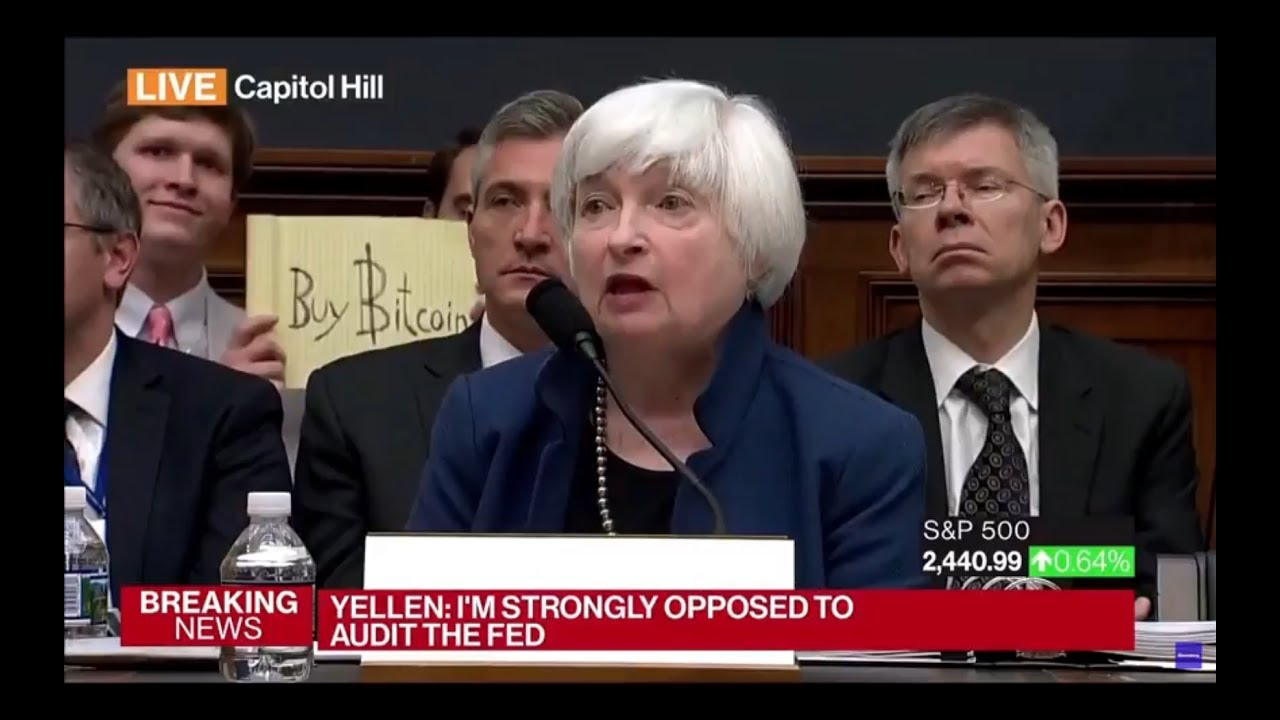
\includegraphics{assets/images/bsg.jpg}
  \caption{Yellen is strongly opposed to audit the Fed, while Bitcoin Sign Guy is strongly in favor to buy bitcoin.}
  \label{fig:bsg}
\end{figure}

While Bitcoin is still inflationary, it will cease to be so rather soon.
The strictly limited supply of 21 million bitcoins will eventually do
away with inflation completely. We now have two monetary worlds: an
inflationary one where money is printed arbitrarily, and the world of
Bitcoin, where final supply is fixed and easily auditable for everyone.
One is forced upon us by violence, the other can be joined by anyone who
wishes to do so. No barriers to entry, no one to ask for permission.
Voluntary participation. That is the beauty of Bitcoin.

I would argue that the argument between Keynesian\footnote{Theories according to
John Maynard Keynes and his deciples~\cite{wiki:keynesian}} and
Austrian\footnote{School of economic thought based on methodological
individualism~\cite{wiki:austrian}} economists is no longer purely academical.
Satoshi managed to build a system for value transfer on steroids, creating the
soundest money which ever existed in the process. One way or another, more and
more people will learn about the scam which is fractional reserve banking. If
they come to similar conclusions as most Austrians and Bitcoiners, they might
join the ever-growing internet of money. Nobody can stop them if they choose to
do so.

\paragraph{Bitcoin taught me that fractional reserve banking is pure insanity.}

% ---
%
% #### Down the Rabbit Hole
%
% - [The Creature From Jekyll Island] by G. Edward Griffin
% - [Money Multiplier][money multiplier], [Keynesian Economics][Keynesian], [Austrian School][Austrian] on Wikipedia
%
% [The Creature From Jekyll Island]: https://archive.org/details/pdfy--Pori1NL6fKm2SnY
%
% [joint debate]: https://www.youtube.com/watch?v=hYzX3YZoMrs
% [money multiplier]: https://en.wikipedia.org/wiki/Money_multiplier
% [auditability]: https://i.ytimg.com/vi/ThFGs347MW8/maxresdefault.jpg
% [Keynesian]: https://en.wikipedia.org/wiki/Keynesian_economics
% [Austrian]: https://en.wikipedia.org/wiki/Austrian_School
%
% <!-- Wikipedia -->
% [alice]: https://en.wikipedia.org/wiki/Alice%27s_Adventures_in_Wonderland
% [carroll]: https://en.wikipedia.org/wiki/Lewis_Carroll
